\makeatletter
\renewcommand*\env@matrix[1][*\c@MaxMatrixCols c]{%
  \hskip -\arraycolsep
  \let\@ifnextchar\new@ifnextchar
  \array{#1}}
\makeatother

\begin{enumerate}
\item The polyhedron is represented as follows:
\begin{center}
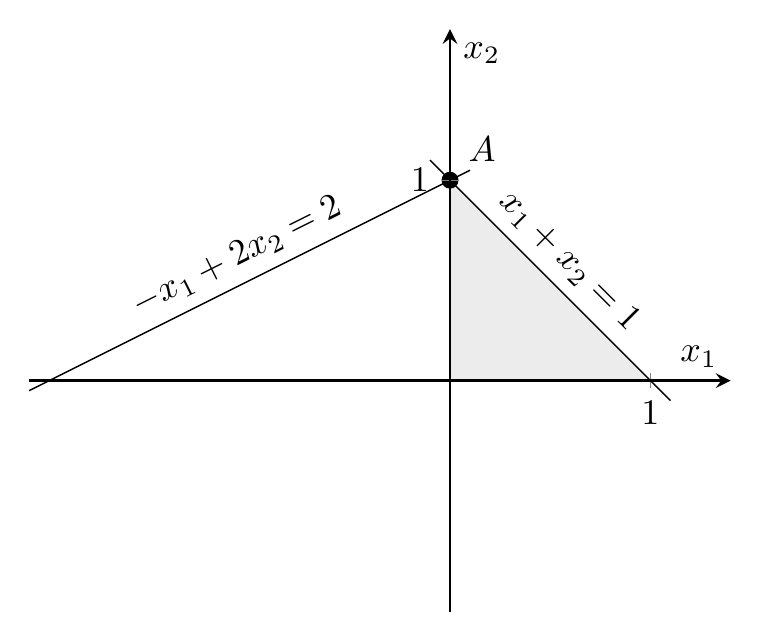
\begin{tikzpicture}[scale=1.3]
\begin{axis}[ xlabel={$x_1$}, ylabel={$x_2$}
    ,axis lines=middle
    ,axis equal
    ,axis on top=true
    ,xtick = {1}
    ,ytick = {1}
,samples=41, thick,
,domain=-0.5:8, xmin=-2.1, xmax=1.4,
    ymin=-0.5, ymax=1.1,
]
\fill[lightgray!30] (0,0) -- (0,1) -- (1,0) -- (0,0) -- cycle;
\addplot+ [mark=none,mark color=black, color=black, thin,domain=-0.1:1.1]{1-x}node[pos=0.5,sloped,above] {$x_1+x_2=1$};
\addplot+ [mark=none,mark color=black, color=black, thin,domain=-2.1:0.1]{1+0.5*x}node[pos=0.5,sloped,above] {$-x_1+2x_2=2$};
\draw (0,5) circle[radius=2.2pt];
\fill (0,5)  circle[radius=2.2pt];
\node [circle,fill=black,draw,scale=0.2,label=above right:$A$] at (0,1) {A};
\end{axis}
\end{tikzpicture}
\end{center}

\item In standard form, after introducing the two slack variables $x_3$ and
$x_4$,  we have
\begin{align*}
x_1+x_2+x_3 & =1,\\
-x_1+2x_2+x_4 &=2,\\
x_1,x_2,x_3,x_4 & \geq 0.
\end{align*}
\item The vertex $A$ corresponds to $x_1=0$, $x_2=1$, $x_3=0$,
$x_4=0$, and is degenerate. Indeed, there are more than $n=2$
constraints that are active at that vertex. There are two active constraints
at each of the two other vertices. Consequently, they are not degenerate.

\item The equality constraints in matrix form are
\[
Ax= b,
\text{ where }
 A \in \mathbb{R}^{2\times 4},\; b \in \mathbb{R}^2,\; x \in \mathbb{R}^4,
\]
\[
A =
\begin{pmatrix*}[r]
1&1&1&0\\
-1&2&0&1
\end{pmatrix*},
b =
\begin{pmatrix*}[r]
1\\
2
\end{pmatrix*}.
\]
We have a problem with $n=4$ variables and $m=2$ equality constraints.
We consider the basic solution where $x_1$ and $x_2$ are in the basis:
$$
B =
\begin{pmatrix*}[r]
1&1\\
-1&2
\end{pmatrix*}
;
B^{-1} =
\begin{pmatrix*}[r]
\frac{2}{3}&-\frac{1}{3}\\
\frac{1}{3} & \frac{1}{3}
\end{pmatrix*}
;
x_B=B^{-1}b=
\begin{pmatrix*}[r]
0\\
1
\end{pmatrix*}
;
x
=
\begin{pmatrix}
0\\
1\\
0\\
0
\end{pmatrix}.
$$
The basic entries of the basic direction corresponding to the non basic variable $x_3$ is
calculated as
\[
-B^{-1} A_3 = -\begin{pmatrix*}[r]
\frac{2}{3}&-\frac{1}{3}\\
\frac{1}{3} & \frac{1}{3}
\end{pmatrix*} \cvect{1 \\ 0} = \cvect{-\frac{2}{3} \\ -\frac{1}{3}}.
\]
Therefore, the basic direction is
\[
d_3 = \cvect{-\frac{2}{3} \\ -\frac{1}{3} \\ 1 \\ 0}.
\]
Moving along $d_3$, we obtain
\[
x^+ = \cvect{0\\
1\\
0\\
0} + \alpha \cvect{-\frac{2}{3} \\ -\frac{1}{3} \\ 1 \\ 0} = \cvect{-\frac{2}{3}\alpha \\ 1-\frac{1}{3}\alpha \\ \alpha \\ 0},
\]
which is infeasible for any $\alpha > 0$. $x_1$ becomes negative as
long as we start following the direction. Therefore, the basic
direction $d_3$ is infeasible. It is represented in the following
figure. 

\begin{center}
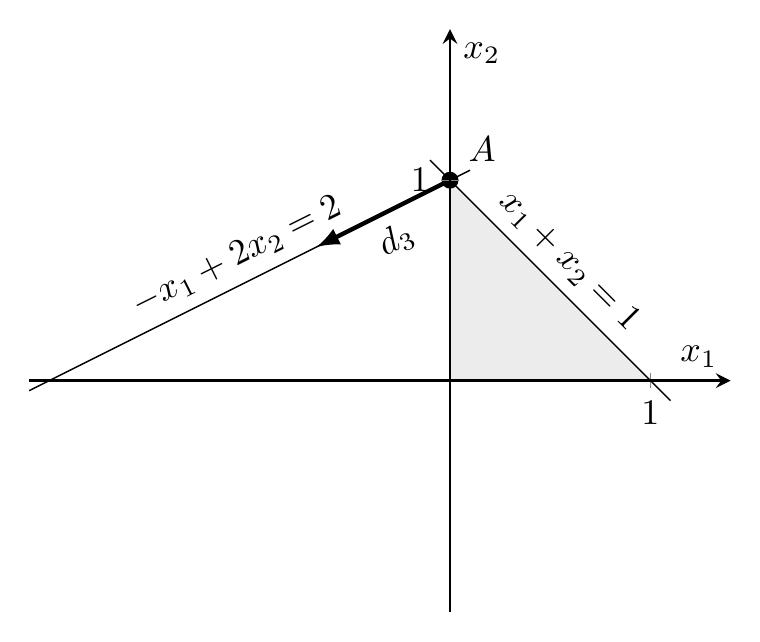
\begin{tikzpicture}[scale=1.3]
\begin{axis}[ xlabel={$x_1$}, ylabel={$x_2$}
    ,axis lines=middle
    ,axis equal
    ,axis on top=true
    ,xtick = {1}
    ,ytick = {1}
,samples=41, thick,
,domain=-0.5:8, xmin=-2.1, xmax=1.4,
    ymin=-0.5, ymax=1.1,
]
\fill[lightgray!30] (0,0) -- (0,1) -- (1,0) -- (0,0) -- cycle;
\addplot+ [mark=none,mark color=black, color=black, thin,domain=-0.1:1.1]{1-x}node[pos=0.5,sloped,above] {$x_1+x_2=1$};
\addplot+ [mark=none,mark color=black, color=black, thin,domain=-2.1:0.1]{1+0.5*x}node[pos=0.5,sloped,above] {$-x_1+2x_2=2$};
\draw (0,5) circle[radius=2.2pt];
\fill (0,5)  circle[radius=2.2pt];
\node [circle,fill=black,draw,scale=0.2,label=above right:$A$] at
(0,1) {A};
\draw[-latex,very thick] (0,1) -- (-2/3,2/3)
node[pos=0.5,below,sloped] {$d_3$};
\end{axis}
\end{tikzpicture}
\end{center}


The basic entries of the basic direction corresponding to the non basic variable $x_4$ is
calculated as
\[
-B^{-1} A_4 = -\begin{pmatrix*}[r]
\frac{2}{3}&-\frac{1}{3}\\
\frac{1}{3} & \frac{1}{3}
\end{pmatrix*} \cvect{0 \\ 1} = \cvect{\frac{1}{3} \\ -\frac{1}{3}}.
\]
Therefore, the basic direction is
\[
d_4 = \cvect{\frac{1}{3} \\ -\frac{1}{3} \\ 0 \\ 1}.
\]
Moving along $d_4$, we obtain
\[
x^+ = \cvect{0\\
1\\
0\\
0} + \alpha \cvect{\frac{1}{3} \\ -\frac{1}{3} \\ 0 \\ 1} =
\cvect{\frac{1}{3}\alpha \\ 1-\frac{1}{3}\alpha \\ 0 \\ \alpha},
\]
which is feasible for $0 \leq \alpha \leq 3$. Therefore, the basic
direction $d_4$ is feasible.
It is represented in the following figure. 

\begin{center}
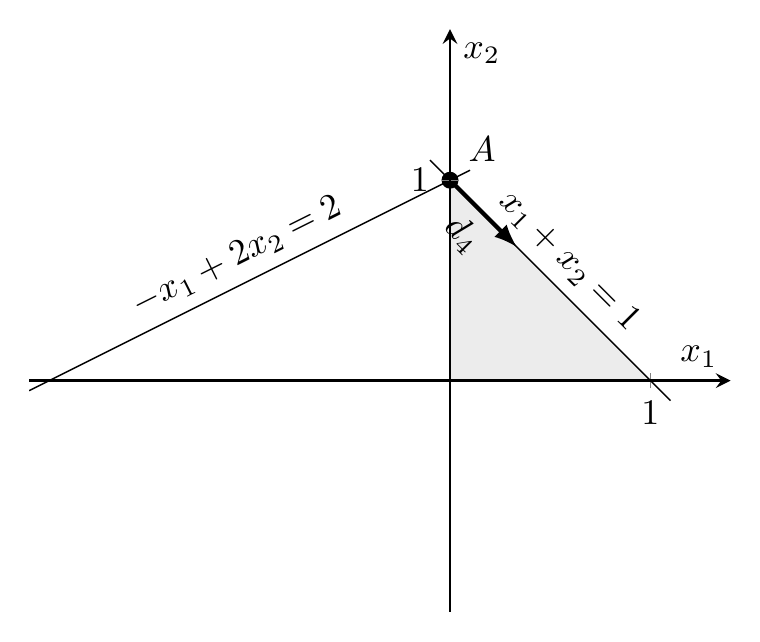
\begin{tikzpicture}[scale=1.3]
\begin{axis}[ xlabel={$x_1$}, ylabel={$x_2$}
    ,axis lines=middle
    ,axis equal
    ,axis on top=true
    ,xtick = {1}
    ,ytick = {1}
,samples=41, thick,
,domain=-0.5:8, xmin=-2.1, xmax=1.4,
    ymin=-0.5, ymax=1.1,
]
\fill[lightgray!30] (0,0) -- (0,1) -- (1,0) -- (0,0) -- cycle;
\addplot+ [mark=none,mark color=black, color=black, thin,domain=-0.1:1.1]{1-x}node[pos=0.5,sloped,above] {$x_1+x_2=1$};
\addplot+ [mark=none,mark color=black, color=black, thin,domain=-2.1:0.1]{1+0.5*x}node[pos=0.5,sloped,above] {$-x_1+2x_2=2$};
\draw (0,5) circle[radius=2.2pt];
\fill (0,5)  circle[radius=2.2pt];
\node [circle,fill=black,draw,scale=0.2,label=above right:$A$] at
(0,1) {A};
\draw[-latex,very thick] (0,1) -- (1/3,2/3)
node[pos=0.5,below,sloped] {$d_4$};
\end{axis}
\end{tikzpicture}
\end{center}

\end{enumerate}
